\documentclass[aspectratio=169,11pt]{beamer}
\usepackage[T1]{fontenc}
\usepackage{lmodern,amsmath,amssymb,booktabs,graphicx}
\definecolor{ink}{HTML}{17324D}
\definecolor{accent}{HTML}{007C83}
\setbeamercolor{normal text}{fg=ink,bg=white}
\setbeamercolor{structure}{fg=accent}
\setbeamercolor{frametitle}{fg=ink}
\setbeamerfont{frametitle}{series=\bfseries,size=\large}
\setbeamertemplate{navigation symbols}{}
\setbeamertemplate{footline}{\hbox to \paperwidth{\hfill\color{ink}\scriptsize ECON 847 \quad Yifan and Wenhan \quad\insertframenumber/\inserttotalframenumber\hspace{5mm}}\vskip3mm}
\setbeamersize{text margin left=8mm,text margin right=8mm}
\newcommand{\source}[1]{\par\vfill{\tiny\color{gray}#1}}
\hypersetup{pdftitle={Bathroom tissue: a conditional merger exercise},pdfauthor={Yifan and Wenhan}}
\begin{document}

\begin{frame}[plain]
\vspace{11mm}
{\LARGE\bfseries Bathroom tissue:\\[3mm]a conditional merger exercise}\par
\vspace{8mm}
{\large Scott and Kimberly-Clark under 1991--1992 conditions}\par
\vspace{9mm}
Yifan and Wenhan\par
ECON 847 \quad November 23, 2026
\end{frame}

\begin{frame}{The counterfactual}
\begin{itemize}\setlength\itemsep{4mm}
\item Combine Scott and Kimberly-Clark's product portfolios in each store-week.
\item Allow manufacturers to reset prices; hold products, costs, demand conditions and retailer rules fixed.
\item Measure price changes, substitution and cost consistency across maintained specifications.
\end{itemize}
\medskip
The firms merged in 1995. Our earlier-period exercise does not reproduce that transaction's timing, remedies or efficiencies.
\source{Sources: v5 design and ownership catalog; SEC, Kimberly-Clark administrative proceeding (April 2002); DOJ merger settlement (December 1995). Full references in SPEAKER\_NOTES.md.}
\end{frame}

\begin{frame}{Industry: portfolios, packaging and a retail chain}
\begin{columns}[T]
\column{.60\textwidth}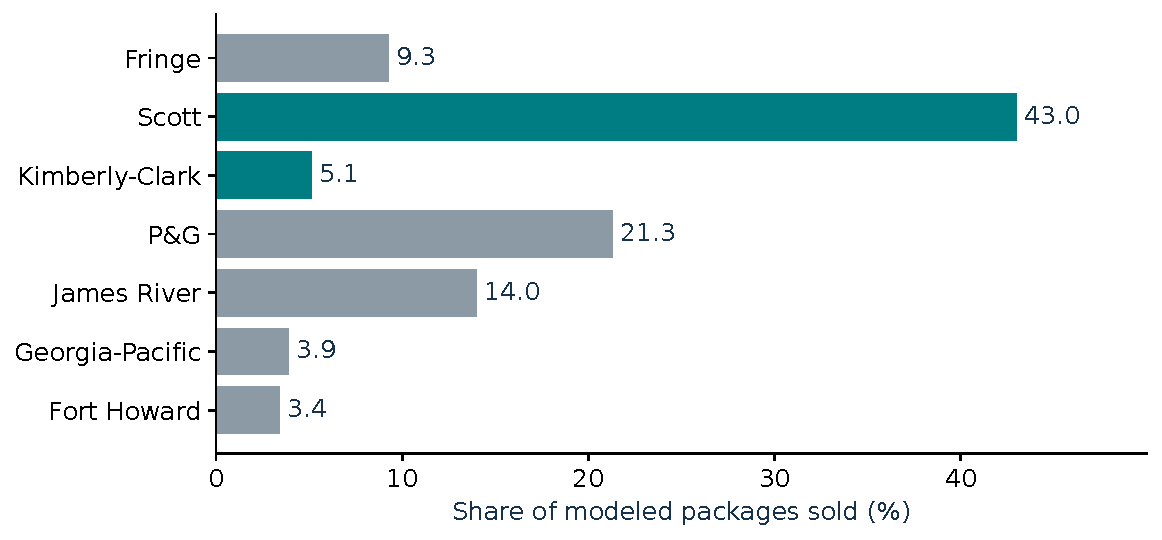
\includegraphics[width=\linewidth]{figures/manufacturers.pdf}
\column{.38\textwidth}\small
Scott: ScotTissue and Cottonelle.\par\medskip
Kimberly-Clark: Kleenex and Delsey.\par\medskip
Products differ in brand and pack size; temporary price reductions are prominent.\par\medskip
Private label/generics remain in demand; their prices stay fixed in the simulation.
\end{columns}
\source{Full estimation sample; shares of modeled packages sold, not national market shares. Ownership: v5 catalog and Hausman--Leonard. Non-anchor prefix grouping is maintained.}
\end{frame}

\begin{frame}{Data and the purchase opportunity}
\begin{columns}[T]
\column{.48\textwidth}
\begin{tabular}{lr}\toprule
Observations & 259,986\\
Store-weeks & 7,996\\
Stores / UPCs & 83 / 50\\
Median UPCs per market & 32\\
Median package price & \$1.15\\
Median AAC proxy & \$0.90\\
Single-roll package volume & 37.7\%\\\bottomrule
\end{tabular}
\column{.48\textwidth}\small
\textbf{Market:} store-week; \textbf{product:} UPC. Retain package differences rather than aggregate brands.\par\medskip
\textbf{Share:} packages sold / weekly shopping trips. Outside: no modeled package purchased on that trip.\par\medskip
Positive-price/share records, complete traffic weeks and saved common keys. Retain 94.31\% of broader-panel packages. True availability and multiple-package purchases remain unobserved.
\end{columns}
\source{Saved v5 product inputs and sample audit. Price/AAC medians are observation-weighted; single-roll volume is package-weighted. Raw data preserved.}
\end{frame}

\begin{frame}{A typical market contains many small product shares}
\centering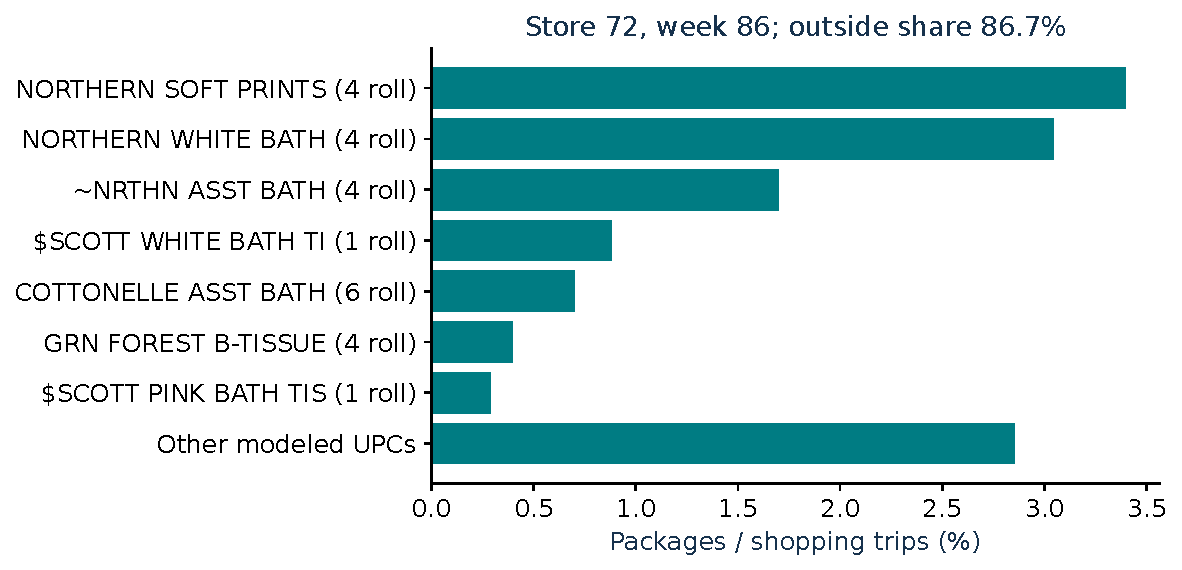
\includegraphics[height=.68\textheight]{figures/typical_market.pdf}
\source{Selected before consulting counterfactual outcomes: nearest to median inside share and product count. Top seven UPCs plus remaining products; the outside option is stated above the chart.}
\end{frame}

\begin{frame}{Temporary price cuts coincide with purchase spikes}
\centering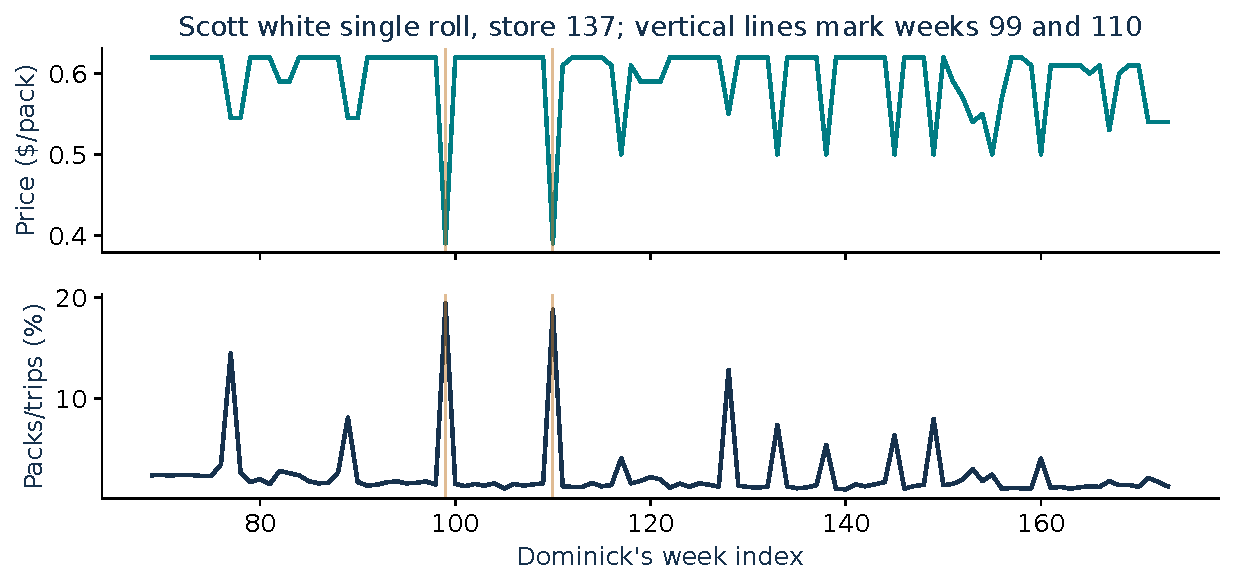
\includegraphics[height=.68\textheight]{figures/promotions.pdf}
\source{Scott white single roll, UPC 5400041500. Store chosen by longest observed series, with store-ID tie break. Missing weeks are not imputed. This is a descriptive association, not a causal promotion estimate.}
\end{frame}

\begin{frame}{Demand and estimation}
For each calibrated nesting parameter $\rho$:
\[
\underbrace{\log(s_{jt}/s_{0t})-\rho\log(s_{jt}/S_t)}_{\text{transformed dependent variable}}
=\alpha_{j,\mathrm{store}}+\tau_t+\beta f(p_{jt})+\gamma\,\mathrm{Deal}_{jt}+\xi_{jt}.
\]
\begin{itemize}\setlength\itemsep{3mm}
\item One inside nest; $S_t=\sum_j s_{jt}$. Linear or log package price: $f(p)=p$ or $\log p$.
\item Absorb store--UPC and week effects; estimate by 2SLS using one excluded price instrument.
\item Conditional inference clusters by store and month; only 24 months.
\item Calibrate $\rho\in\{0,.25,.50,.75\}$; the instrument does not jointly identify price sensitivity and nesting.
\end{itemize}
\source{v5 methods; the fixed effects absorb persistent store/product quality and common weekly shocks. Time-varying local demand shocks remain in the error.}
\end{frame}

\begin{frame}{Price instruments predict prices, but exclusion is assumed}
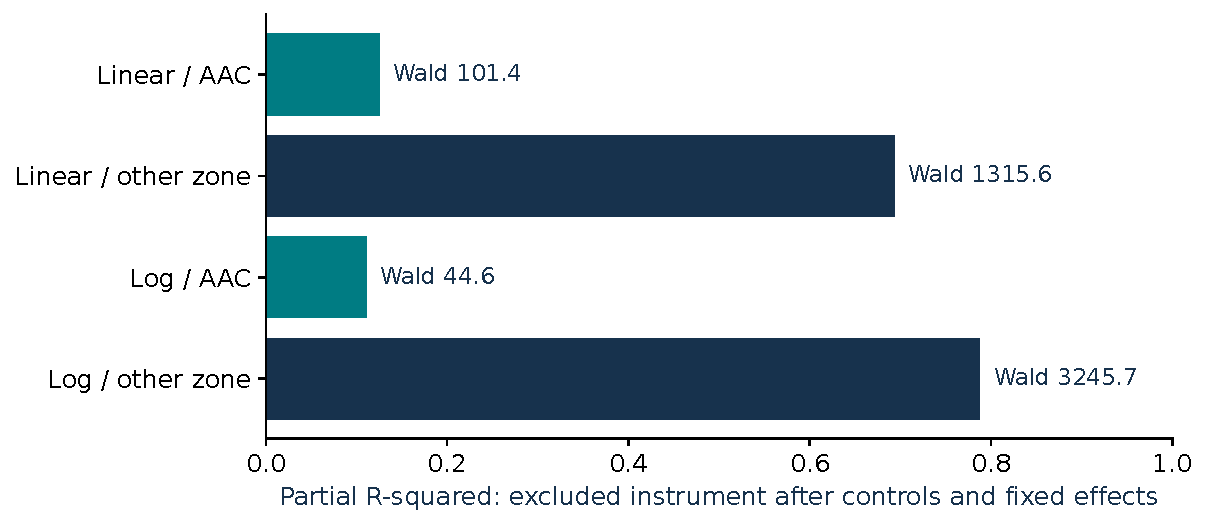
\includegraphics[width=.94\textwidth,height=.43\textheight,keepaspectratio]{figures/first_stages.pdf}\par
\small
AAC: acquisition-cost proxy; may correlate with promotions or demand shocks.\par\smallskip
Other-zone price: common costs can help; common demand shocks can invalidate it.\par\smallskip
Maintain $E[\widetilde z\,\xi]=0$ after controls; log-price cells use log instruments and need their own moment restriction. Deal is treated as exogenous.
\source{Saved conditional first stages, same sample. Wald chi-square is not an effective-F statistic. One excluded IV: no overidentification degrees of freedom.}
\end{frame}

\begin{frame}{Supply and counterfactual assumptions}
\small
\begin{enumerate}\setlength\itemsep{2.6mm}
\item Manufacturers maximize static portfolio profit: $\sum_{j\in f}(q_jp_j-c_j)s_j(p)$; named rivals also reoptimize.
\item Dollar retailer margins: $q_j=1$, and $c_j$ is retail-equivalent cost. Percentage margins: $q_j=1-m_j$, and $c_j$ is manufacturer cost.
\item Invert baseline first-order conditions for costs, then change ownership. No efficiencies, entry, exit, assortment changes or inventories.
\item Hold market size, non-price utilities, deal and retailer rule fixed; fringe prices remain observed.
\item Report price effects on common numerical markets. Report cost signs on the full input sample; retain failures rather than clip costs.
\end{enumerate}
\source{v5 supply design. Dollar-rule manufacturer-cost diagnostic uses AAC minus markup; percentage costs use calibrated q times price minus markup.}
\end{frame}

\begin{frame}{Rho-zero results: four demand cells, two retailer rules}
\centering\small
\begin{tabular}{lrrrr}\toprule
&\multicolumn{2}{c}{Dollar margins}&\multicolumn{2}{c}{Percentage margins}\\
&Category&K--C&Category&K--C\\\midrule
Linear / AAC & 0.38 & 2.82 & 0.37 & 3.12 \\
Linear / other zone & 0.28 & 2.13 & 0.28 & 2.36 \\
Log / AAC & 0.16 & 1.03 & 0.16 & 1.13 \\
Log / other zone & 0.17 & 1.08 & 0.16 & 1.18 \\
\bottomrule\end{tabular}
\par\medskip\normalsize
Baseline-package-weighted price changes (\%).\par\medskip
These scenarios provide an accessible starting comparison. Better cost signs do not select a preferred demand model.
\source{Common numerical sample: 7,960 markets, 97.08\% of baseline packages. Negative-cost cases included. K--C = Kimberly-Clark. Scenario comparisons are not confidence intervals.}
\end{frame}

\begin{frame}{Nesting moves merger predictions most over this grid}
\centering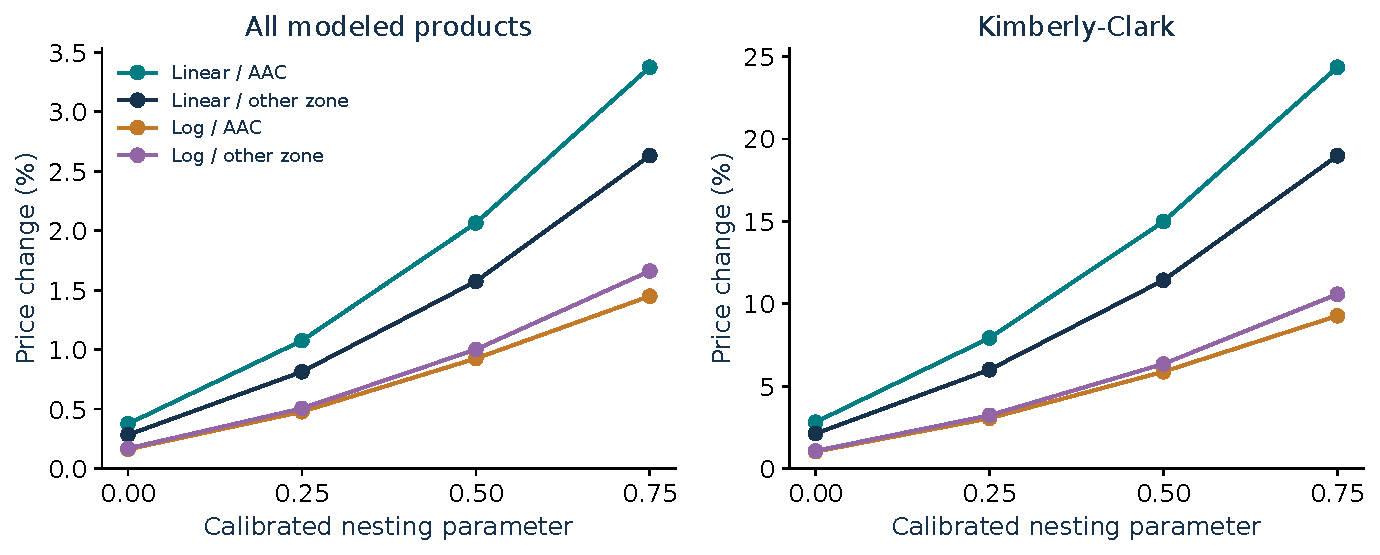
\includegraphics[width=.98\textwidth]{figures/price_sensitivity.pdf}\par
\small
Largest matched changes: nesting about 3.0 percentage points for category prices and 21.5 for K--C; price form about 1.9 and 15.1. Instrument and rho-zero retailer-rule changes are smaller.
\source{Dollar-margin curves; common numerical sample. Compare one assumption at a time holding the others fixed. Ranking depends on the tested grid; it is not a causal variance decomposition.}
\end{frame}

\begin{frame}{Negative implied costs are an economic result}
\centering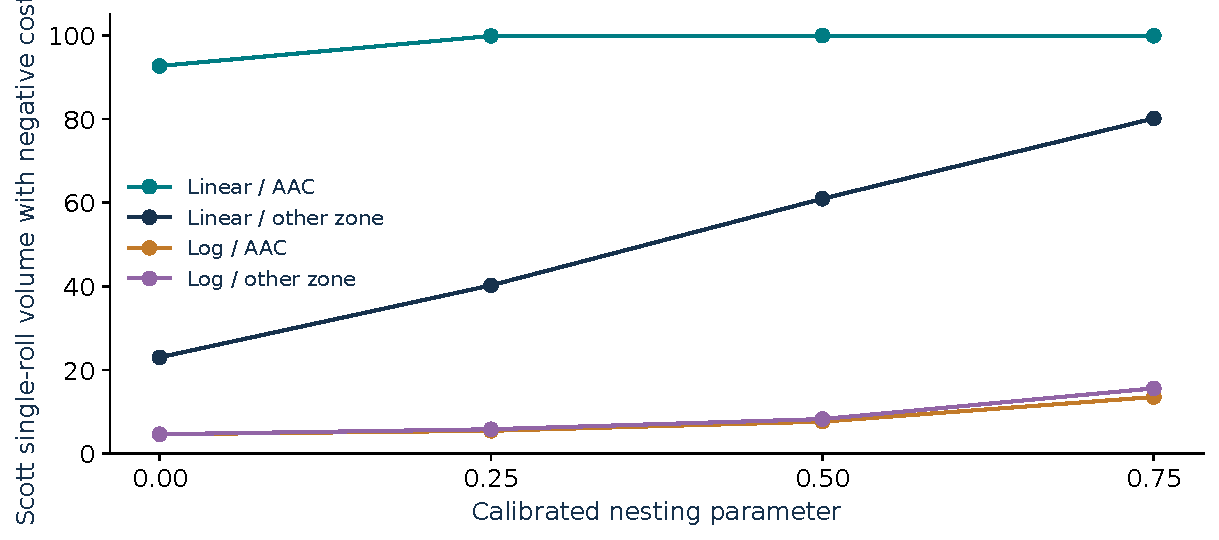
\includegraphics[height=.58\textheight]{figures/cost_failures.pdf}\par
\small
Including percentage sensitivities: linear/AAC 62--100\%, linear/other-zone 21--80\%, log price 3--16\% of Scott single-roll volume.
\source{Full input sample; denominator is Scott single-roll packages. Curves show dollar margins. Accepted-sample zeros are not independent cost validation. Frozen cost diagnosis, REVIEW-005.}
\end{frame}

\begin{frame}{The model is strained by cheap single rolls}
\begin{itemize}\setlength\itemsep{3.5mm}
\item Linear/AAC own elasticity is about $-1.0$ for single rolls; log/AAC gives about $-5.2$. Portfolio pricing increases recovered markups further.
\item Deep-discount rows supply 56\% of the log/AAC instrument--price cross-product, despite being 23\% of rows.
\item High-purchase-share episodes are hardest for baseline numerical recovery. A package-per-trip share may not describe a single consumer choice during such episodes.
\item These facts motivate inventory and quantity-choice models; they do not identify stockpiling or prove a particular replacement model.
\end{itemize}
\source{Elasticities: common numerical sample, package-weighted, all single rolls. Discount: more than 5\% below store--UPC modal price. Moment contribution is descriptive, not a causal estimate.}
\end{frame}

\begin{frame}{What the exercise teaches about counterfactuals}
\begin{itemize}\setlength\itemsep{4mm}
\item Substitution assumptions move merger predictions substantially even when own elasticities appear stable across nesting values.
\item Cost inversion links demand, portfolio ownership and retailer assumptions. Negative costs expose tension among those assumptions.
\item Strong first stages and solver success cannot establish identification. Earlier mixed-logit attempts did not resolve the concerns.
\item Better purchase-unit/availability measurement and a credible source of price variation are priorities for a subsequent model.
\end{itemize}
\source{The current exercise is complete. Aggregation or dynamic modeling would change the research question and needs separate justification.}
\end{frame}

\begin{frame}{Conclusions and discussion}
\large
The maintained scenarios predict price increases after the merger.\par\medskip
The magnitude depends strongly on nesting and price functional form.\par\medskip
Cost failures show where a static package-choice model and manufacturer pricing cease to be convincing.\par\bigskip
\normalsize
\textbf{Discussion:} which measurement or identifying assumption would you change first, and what new evidence would make that change credible?
\end{frame}
\end{document}
